\documentclass[12pt]{book}
\usepackage{caption}
\usepackage{subcaption}
\usepackage{minitoc}
\usepackage{minitoc}
\usepackage{lipsum}
\usepackage{xcolor}
\usepackage[french]{babel}
\usepackage{ragged2e}
\usepackage{tabularx}
\usepackage{multirow}
\usepackage{pdfpages}

% Change the caption font in italic
\renewcommand{\captionfont}{\it}

%%%%%%%%%%%%%%%%%%%%%%%%%%%% biblio
\usepackage[round]{natbib}

%%%%%%%%%%%%%%%%%%%%%%%%%%%% Margins
\usepackage{geometry}
\geometry{top=3cm, bottom=3cm, left=3cm, right=3cm}

%%%%%%%%%%%%%%%%%%%%%%%%%%%% Double spaced lines
\usepackage{setspace}
\doublespacing

%%%%%%%%%%%%%%%%%%%%%%%%%%%% Line numbers
\usepackage{lineno}
\linenumbers

%%%%%%%%%%%%%%%%%%%%%%%%%%%% Header/footer definition
\usepackage{fancyhdr}

%%%%%%%%%%%%%%%%%%%%%%%%%%% For toc management
\setcounter{tocdepth}{1}
\setcounter{minitocdepth}{6}

%%%%%%%%%%%%%%%%%%%%%%%%%% reference (must be loaded after minitoc)
\usepackage{hyperref}

\hypersetup{
    colorlinks = true,
    linkcolor=,
    urlcolor = blue,
    citecolor=black
}
%%%%%%%%%%%%%%%%%%%%%%%%%%%%%%% Define homemade style for header/footer
% Redefine commands of chapter and section writting
% Hard to understand, even for me

% Original format
% \renewcommand{\chaptermark}[1]{\markboth{\MakeUppercase{\chaptername\ \thechapter.\ #1}}{}}
% \renewcommand{\sectionmark}[1]{\markright{\MakeUppercase{\thesection .\ #1}}{}}

% New format
\renewcommand{\chaptermark}[1]{\markboth{\textit{\chaptername\ \thechapter.\ #1}}{}}
\renewcommand{\sectionmark}[1]{\markright{\textit{\thesection .\ #1}}{}}

%%%%%%%%%%%% define a fancy style for headers
\fancypagestyle{mystyle} {
\fancyhead{} % clear all header fields

% Modify the header methods
\fancyhead[RO]{\rightmark} % chapter for right odd page header
\fancyhead[LE]{\leftmark} % section for left even page header

\fancyfoot[RO]{Nicolas Barrier} % author for right odd footer
\fancyfoot[LE]{2 Septembre 2024} % date for left even footer
}

%%%%%%%%%%%%%%%%%%%%%%%%%%%%%%%%%%%%%%%%%%% Renaming figures/equations/tables
\makeatletter
\renewcommand\theequation{\thechapter.\arabic{equation}}
\@addtoreset{equation}{chapter}
\makeatother

\makeatletter
\renewcommand\thefigure{\thechapter.\arabic{figure}}
\@addtoreset{figure}{chapter}
\makeatother

\makeatletter
\renewcommand\thetable{\thechapter.\arabic{table}}
\@addtoreset{table}{chapter}
\makeatother    

\title{My PhD Thesis}
\author{Nicolas Barrier}
\date{\today}

\begin{document}

% Include a PDF page
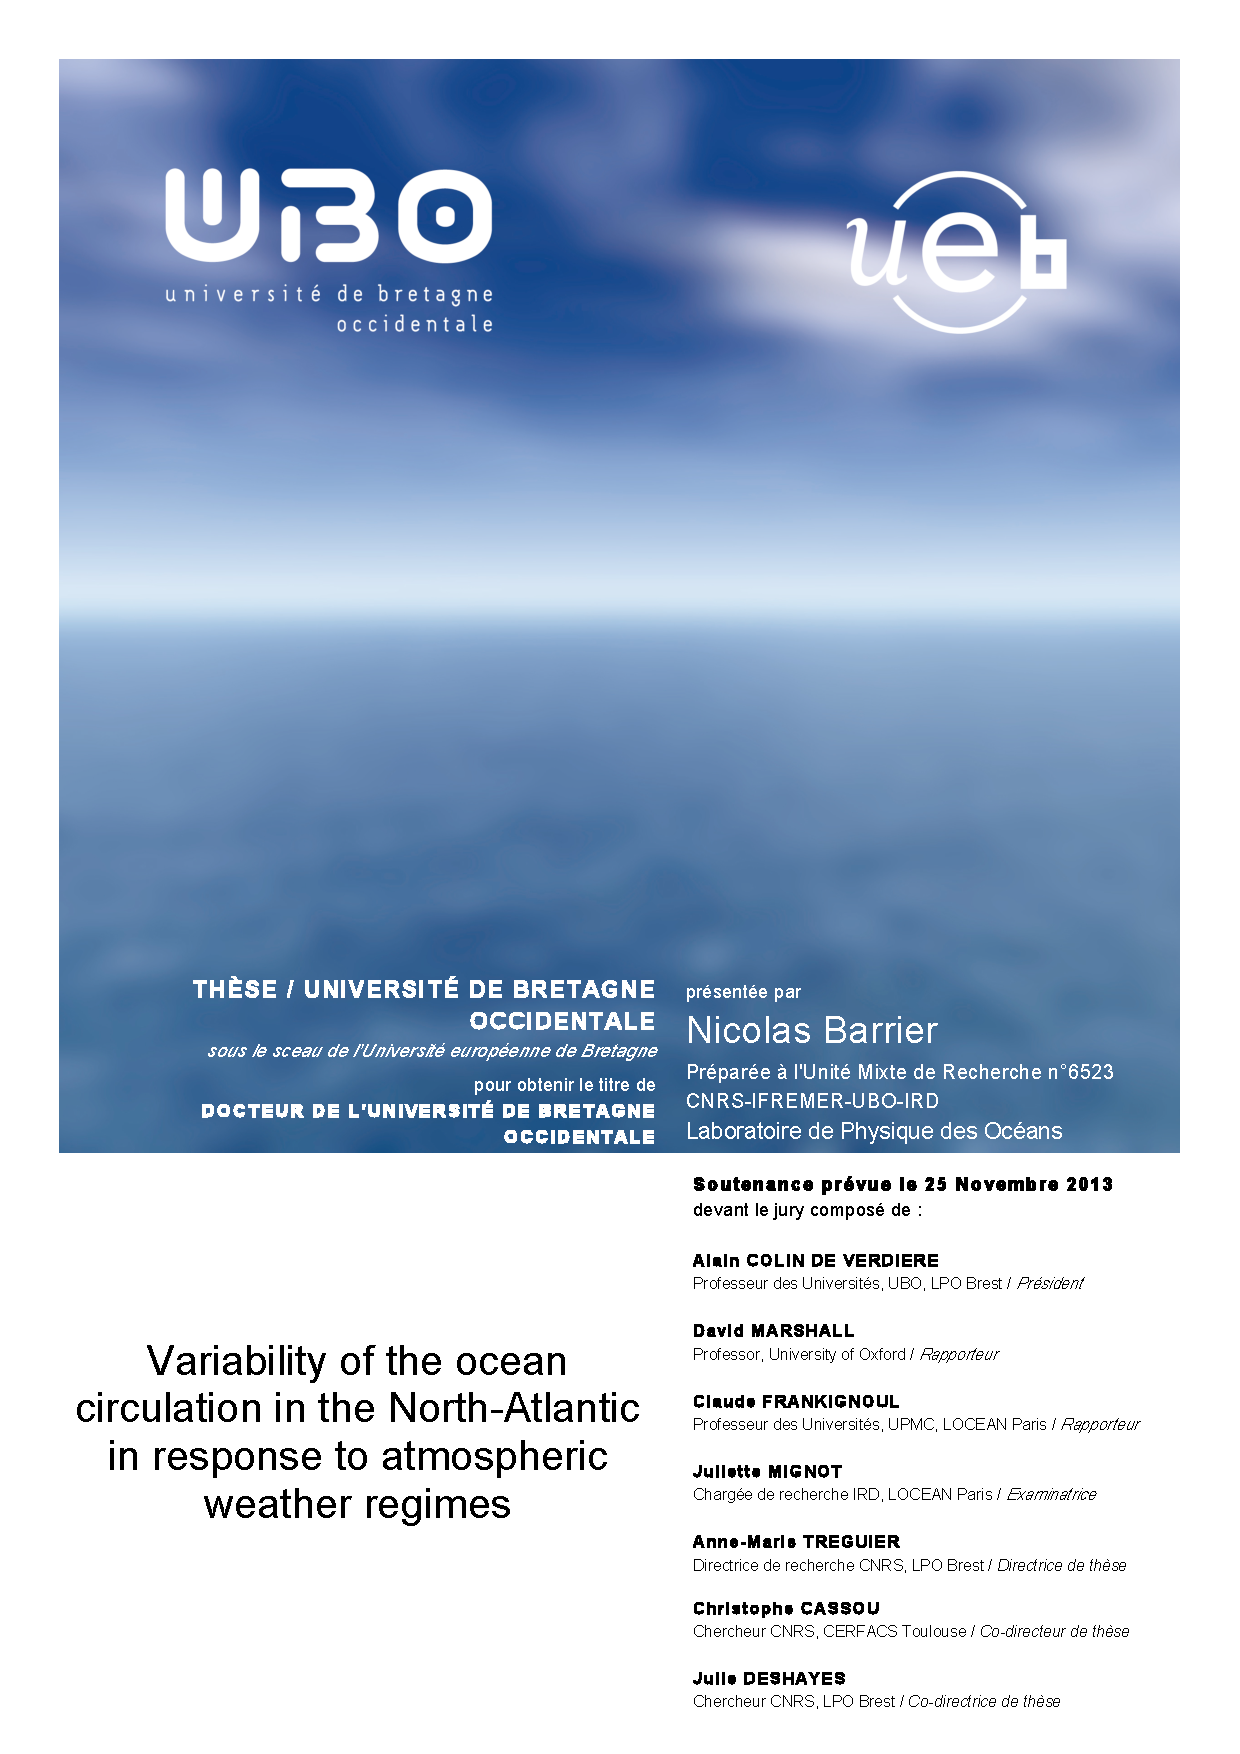
\includepdf[pages=-]{figs/Couverture_nbarrier.pdf}
% or use the \maketitle instead
\maketitle

% For activating Mini TOC
\dominitoc

% set empty page style for the table of content (no header/footer)
\pagestyle{empty} 
\tableofcontents

\clearpage

% set the pagestyle for the remaining of the document
\pagestyle{mystyle}

\chapter{Introduction}
\addstarredchapter{Introduction}
\minitoc
\lipsum
\section{Context}
\lipsum

\begin{figure}[h!]
    \centering
    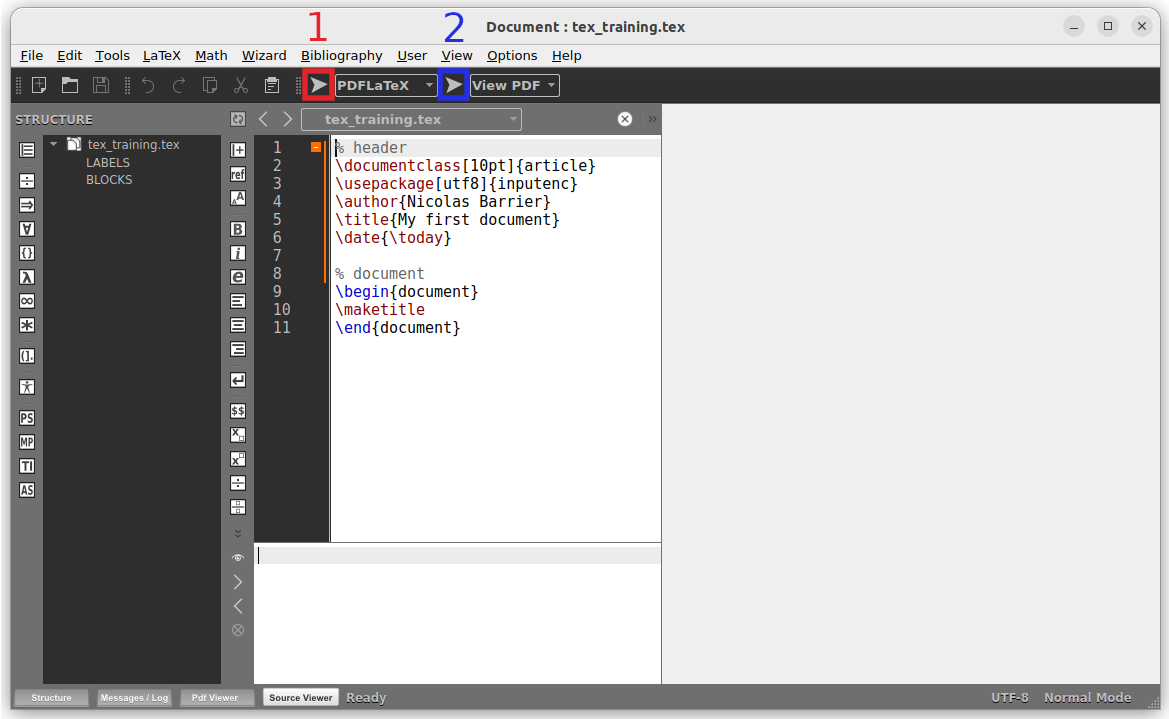
\includegraphics[width=0.5\linewidth]{figs/texmaker-1.png}
    \caption{Compilation using Texmaker}
\end{figure}


\section{Outline}


\chapter{Data and method}
\label{chap:data-method}
\minitoc

\section{Data}
\subsection{Data subsection}
\subsubsection{Data sub-sub section}
\lipsum[1-3]

\begin{figure}[h!]
    \centering
    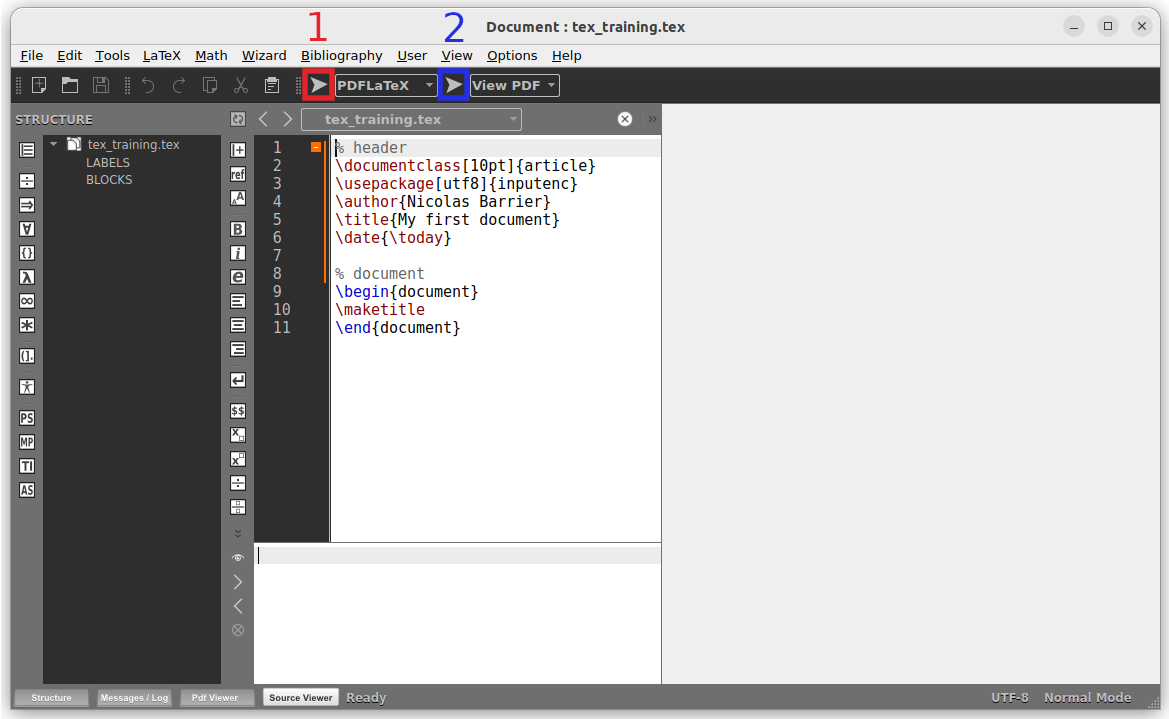
\includegraphics[width=0.5\linewidth]{figs/texmaker-1.png}
    \caption{Compilation using Texmaker}
\end{figure}

\lipsum[4-7]

\section{Method}

\lipsum[1-5]

\begin{figure}[h!]
    \centering
    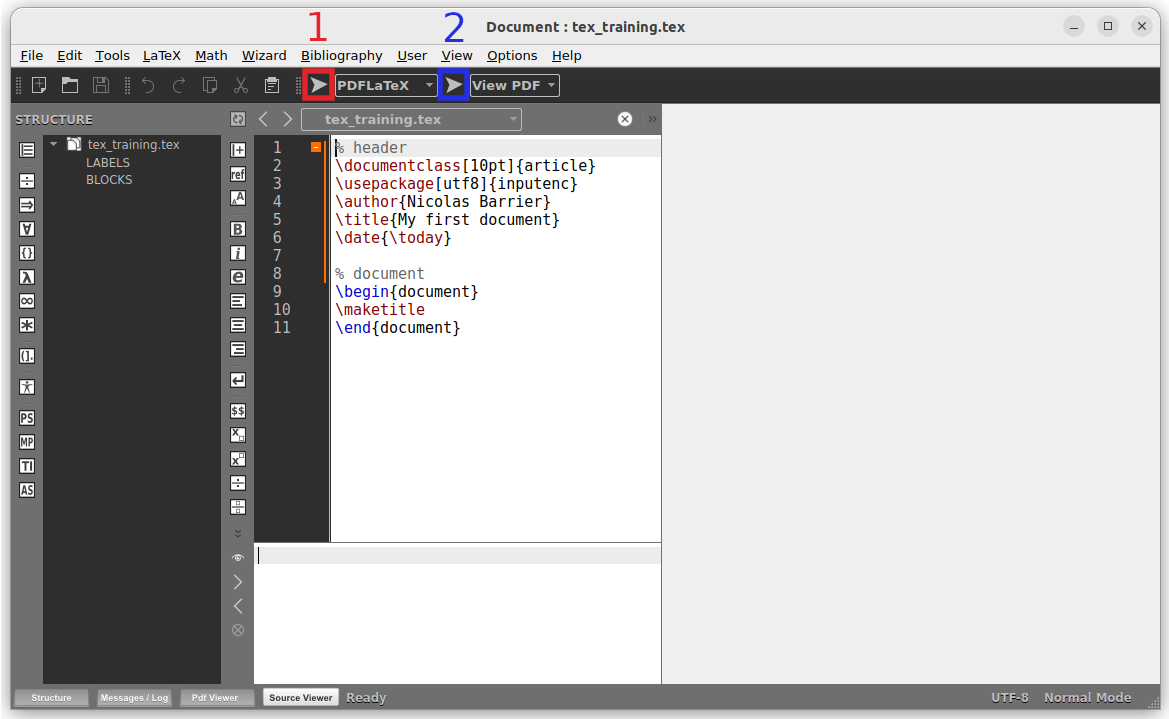
\includegraphics[width=0.5\linewidth]{figs/texmaker-1.png}
    \caption{Compilation using Texmaker}
\end{figure}

\lipsum[6-7]

\chapter{Results}
\minitoc

\chapter{Conclusion}
\addstarredchapter{Conclusion}
\minitoc
\section{Conclusion}
\lipsum

\section{Discussion}
\lipsum

\section{Perspectives}
\lipsum


\lipsum[1-4]

\chapter*{References}
\addstarredchapter{References}

\nocite{*}
\bibliographystyle{plainnat} % We choose the "plain" reference style
\bibliography{biblio.bib} % Entries are in the refs.bib file

\end{document}